%%%%%%%%%%%%%%%%%%%%%%% file template.tex %%%%%%%%%%%%%%%%%%%%%%%%%
%
% This is a general template file for the LaTeX package SVJour3
% for Springer journals.          Springer Heidelberg 2010/09/16
%
% Copy it to a new file with a new name and use it as the basis
% for your article. Delete % signs as needed.
%
% This template includes a few options for different layouts and
% content for various journals. Please consult a previous issue of
% your journal as needed.
%
%%%%%%%%%%%%%%%%%%%%%%%%%%%%%%%%%%%%%%%%%%%%%%%%%%%%%%%%%%%%%%%%%%%
%
% First comes an example EPS file -- just ignore it and
% proceed on the \documentclass line
% your LaTeX will extract the file if required
\begin{filecontents*}{example.eps}
%!PS-Adobe-3.0 EPSF-3.0
%%BoundingBox: 19 19 221 221
%%CreationDate: Mon Sep 29 1997
%%Creator: programmed by hand (JK)
%%EndComments
gsave
newpath
  20 20 moveto
  20 220 lineto
  220 220 lineto
  220 20 lineto
closepath
2 setlinewidth
gsave
  .4 setgray fill
grestore
stroke
grestore
\end{filecontents*}
%
\RequirePackage{fix-cm}
%
%\documentclass{svjour3}                     % onecolumn (standard format)
%\documentclass[smallcondensed]{svjour3}     % onecolumn (ditto)
\documentclass[smallextended,envcountsame]{svjour3}       % onecolumn (second format)
%\documentclass[twocolumn]{svjour3}          % twocolumn
%
\smartqed  % flush right qed marks, e.g. at end of proof
%
\usepackage{graphicx}
%
\usepackage{mathptmx}      % use Times fonts if available on your TeX system
%
% insert here the call for the packages your document requires
%\usepackage{latexsym}

\usepackage{amsmath}
\usepackage{amsfonts}
\usepackage{amssymb}
\usepackage{eurosym}
\usepackage{mathtools}
\usepackage{graphicx}
\usepackage{rotating}
\usepackage{setspace}
\usepackage{color}
\usepackage{fancyhdr}
\usepackage{ragged2e}
\usepackage{appendix}
\usepackage{tabularx}
\usepackage{multirow}
\usepackage{booktabs}
\usepackage{xfrac}
\usepackage{pgfplots}
\usepackage{url}
\usepackage{emptypage}
\usepackage{wrapfig}
\usepackage{dsfont}
\usepackage{soul}
\usepackage{tikz}
\usetikzlibrary{arrows.meta, positioning}

% \usepackage[backend=bibtex,style=alphabetic]{biblatex}
% \addbibresource{sample.bib}

\usepackage{csquotes}
\usepackage{hyperref}

% \usepackage[
%   backend=biber,
%   style=alphabetic,
%   sorting=nty,
%   maxbibnames=99,
%   url=false,  % Exclude URLs
%   % issn = false
%   %doi=false,   % Exclude DOIs
%   %isbn=false
% ]{biblatex}

% \addbibresource{sample.bib}
%
% please place your own definitions here and don't use \def but
% \newcommand{}{}


\usepackage{xcolor}
\usepackage{todonotes}
\newcommand{\gr}[2][]{\todo[color=violet!40!,#1]{\textsf{GR:} #2}}
\newcommand{\bm}[2][]{\todo[color=blue!20,#1]{\textsf{BM:} #2}}

%\newtheorem{example}{Example}
\newtheorem{assumption}{Assumption}
%\newtheorem{definition}{Definition}
%\newtheorem{theorem}{Theorem}
%\newtheorem{corollary}{Corollary}[theorem]
%\newtheorem{lemma}[theorem]{Lemma}
\newtheorem{prop}[theorem]{Proposition}
\newtheorem{observation}[theorem]{Observation}
%\newtheorem{problem}{Problem}

\DeclareMathOperator{\diag}{diag}
\DeclareMathOperator{\dw}{d_w}
\DeclareMathOperator{\C}{C_{tc}}
\DeclareMathOperator{\T}{T}
\DeclareMathOperator{\MP}{MP}
\DeclareMathOperator{\KP}{KP}
\DeclareMathOperator{\K}{K}
\DeclareMathOperator{\Id}{Id}
\DeclareMathOperator{\SSpan}{Span}
%\DeclareMathOperator{\lim}{lim}
\DeclareMathOperator{\epi}{epi}
\DeclareMathOperator{\supp}{supp}


%\numberwithin{definition}{section}
\numberwithin{theorem}{section}
%\numberwithin{problem}{section}
\newcommand{\nc}{\newcommand}
\nc{\boB}{{\mathbf{B}}}
\nc{\boL}{{\mathbf{L}}}
\nc{\boY}{{\mathbf{Y}}}
\nc{\boI}{{\mathbf{I}}}
\nc{\boV}{{\mathbf{V}}}
\nc{\boS}{{\mathbf{S}}}
\nc{\tV}{{\Tilde{{V}}}}
\nc{\tI}{{\Tilde{{I}}}}
\nc{\tY}{{\Tilde{{Y}}}}
\nc{\tS}{{\Tilde{{S}}}}
\nc{\fr}{{\rightarrow}}
\nc{\co}{{\nabla}}
\nc{\E}{\mathbb{E}}
\nc{\CG}{C_{\Sigma}^{\text{Gauss}}}
\nc{\var}{Var}
\nc{\rows}{S}
\nc{\cols}{R}
\nc{\rowP}{\sigma}
\nc{\colP}{\delta}
\nc{\rowW}{\omega}
\nc{\colW}{\tau}

\nc{\sS}{ \mathscr{S}}
\nc{\sC}{ \mathscr{C}}
\nc{\cH}{{\mathcal H}}
\nc{\cR}{{\mathcal R}}
\nc{\cA}{{\mathcal A}}
\nc{\cG}{{\mathcal G}}
\nc{\cC}{{\mathcal C}}
\nc{\cD}{{\mathcal D}}
\nc{\cO}{{\mathcal O}}
\nc{\cI}{{\mathcal I}}
\nc{\cB}{{\mathcal B}}
\nc{\cY}{{\mathcal Y}}
\nc{\cK}{{\mathcal K}} 
\nc{\cX}{{\mathcal X}}
\nc{\cS}{{\mathcal S}}
\nc{\cE}{{\mathcal E}}
\nc{\cF}{{\mathcal F}}
\nc{\cZ}{{\mathcal Z}}
\nc{\cQ}{{\mathcal Q}}
\nc{\cP}{{\mathcal P}}
\nc{\cL}{{\mathcal L}}
\nc{\cM}{{\mathcal M}}
\nc{\cN}{{\mathcal N}}
\nc{\cT}{{\mathcal T}}
\nc{\cW}{{\mathcal W}}
\nc{\cU}{{\mathcal U}}
\nc{\cJ}{{\mathcal J}}
\nc{\cV}{{\mathcal V}}
\nc{\bH}{{\mathbb H}}
\nc{\bA}{{\mathbb A}}
\nc{\bG}{{\mathbb G}}
\nc{\bC}{{\mathbb C}}
\nc{\bO}{{\mathbb O}}
\nc{\bI}{{\mathbb I}}
\nc{\bB}{{\mathbb B}}
\nc{\bY}{{\mathbb Y}}
\nc{\bK}{{\mathbb K}} 
\nc{\bX}{{\mathbb X}}
\nc{\bS}{{\mathbb S}}
\nc{\bE}{{\mathbb E}}
\nc{\bF}{{\mathbb F}}
\nc{\bZ}{{\mathbb Z}}
\nc{\bQ}{{\mathbb Q}}
\nc{\bN}{{\mathbb N}}
\nc{\bP}{{\mathbb P}}
\nc{\bL}{{\mathbb L}}
\nc{\bM}{{\mathbb M}}
\nc{\bT}{{\mathbb T}}
\nc{\bW}{{\mathbb W}}
\nc{\bU}{{\mathbb U}}
\nc{\bD}{{\mathbb D}}
\nc{\bJ}{{\mathbb J}}
\nc{\bV}{{\mathbb V}}
\nc{\bR}{{\mathbb R}}


\newcommand{\virgolette}[1]{``#1''} %\virgolette{questo č fra virgolette}%
%\usepackage{frontespizio}
\newcommand{\abs}[1]{\lvert#1\rvert}



%
% Insert the name of "your journal" with
\journalname{Optimization and Engineering}
%
\begin{document}

\title{Modelling of a fully renewable energy grid with hydrogen storage: time aggregation for a scalable Capacity Expansion Problem
%\thanks{Grants or other notes
%about the article that should go on the front page should be
%placed here. General acknowledgments should be placed at the end of the article.}
}
\subtitle{}%A stochastic approach considering time interdependence of wind and solar power.}

%\titlerunning{Short form of title}        % if too long for running head

\author{Bianca Urso         \and
        Gabor Riccardi %etc.
}

%\authorrunning{Short form of author list} % if too long for running head

\institute{B. Urso \at
              IUSS School of Advances Studies, Palazzo del Broletto, Piazza della Vittoria, 15 – 27100 Pavia PV, Italy\\
              Tel: +39 0382 375811\\
              Fax: +39 0382 375899\\
              \email{bianca.urso@iusspavia.it}           %  \\
%             \emph{Present address:} of F. Author  %  if needed
           \and
           G. Riccardi \at
           Dipartimento di Matematica ”F. Casorati”
           Via Adolfo Ferrata, 5 – 27100 Pavia
}

\date{Received: date / Accepted: date}
% The correct dates will be entered by the editor


\maketitle

\begin{abstract}
In recent years, the integration of renewable energy sources into electrical grids has become a
critical area of research due to the increasing need for sustainable
and resilient energy systems.  To adress the variability of wind and solar power output over time, electricity grids expansion plans need to account for multiple scenarios over large time horizons.
This significanlty increases the size of the resulting Linear Problem (LP), making them computationally challenging for large scale grids.
To tackle this, we propose an approach that aggregates time steps to reduce the problem size, followed by an iterative refinement of the aggregation. 
\textcolor{violet}{We provide sufficient conditions under which the aggregated problem is equivalent to the original, unaggregated one, and refine the time intervals that do not meet these conditions.
\textbf{write better:Additionally, we introduce a validation function to assess the feasibility of the aggregated solutions. Our method is tested on a fully renewable energy grid with hydrogen storage.}
 We generate scenarios for wind and photovoltaic (PV) power output using scenario generation techniques that capture temporal dependencies. 
 These dependencies are modeled with marginal distributions coupled with a Gaussian copula, ensuring that the generated scenarios reflect realistic 
 temporal correlations observed in historical data.}
%Insert your abstract here. Include keywords, PACS and mathematical
%subject classification numbers as needed.
\keywords{\textcolor{red}{First keyword \and Second keyword \and need 4-6}}
% \PACS{PACS code1 \and PACS code2 \and more}
\subclass{90-10 \and 90B15 }
\end{abstract}

\newpage
\section{INTRODUCTION}

\textbf{Context; literature overview. Small introduction on LP/MIP. Definition of stochastic optimization,
definition of CEP, ED problems.}\\


The threat of climate change is pushing policy-makers to pursue greater integration of renewable energy sources into electrical grids, while at the same time ensuring reliability and resilience through digital optimization of electric power distribution and transmission in smart grids \textcolor{green}{\cite{EU_context}}. One of the main difficulties arising when designing an electric power system relying on renewables is the great variability of the generation of electricity through wind and solar, since these resources are highly dependent on weather conditions, \textcolor{red}{curtailment = inefficient, need hydrogen, cite source for hydrogen (eg: EU super investing in it). The stochastic nature of the problem....} making it impossible to plan long-term by optimizing on forecasts, and requiring a statistical approach to ensure a robust model.
Up to now, common approaches have adopted Stochastic Programming (SP) or Robust Optimization (RO) models, along with hybrid models involving Information Gap Decision Theory or Chance Constraint \textcolor{green}{\cite{review_math_opt}}. While initially favored, the SP approach comes with high computational burden, so RO models have seen more popularity in recent years, despite the drawback of being conservative methods with higher average cost of operation and planning of energy systems.\\
\indent In the typical setting, the problem to solve is a Capacity Expansion Problem (CEP) regarding infrastructure investments: solar and wind farms, fuel cells, hydrolizers, grid upgrades to augment Net Transfer Capacity (NTC) and so on. Nested within the CEP is an Economic Dispatch (ED) problem concerning the operational costs of said infrastructure. 
The problem is well suited to be modelled through mixed integer linear programming (MILP), as is explained in detail in \textcolor{green}{\cite{INTRO_isolated_MIP}} and ((\textcolor{red}{other examples?}))\\
\indent The CEP for investment planning requires to look at long time horizons, and on the other hand intra-day variability in generation \textcolor{pink}{is the main complexity driver} for the ED problem, so the time horizon must be modelled by a large quantity of fairly tight time steps. Furthermore, \textcolor{pink}{spacial structure big, even though we ignore it here and just slam everything into country nodes}. 
Thus the temporal and spacial characteristics of the model bring the MILP size to increase rapidly. This is especially demanding in the case of SP, since all the variables from the inner ED problem must be reproduced over all scenarios.\\
\indent To reduce these costs, one possible approach is to use a Rolling Horizon (RH) \textcolor{red}{[explain better]}. The basic technique is described in \textcolor{green}{\cite{INTRO_Glomb}}, along with some results regarding quality guarantees for the optimality of the solution. In \textcolor{green}{\cite{INTRO_Palma-Behnke}}, a rolling horizon approach is used within a RO model to optimize the operation of a micro-grid composed of \textcolor{pink}{check} serving an isolated area in Chile. \textcolor{red}{other examples of RH used for the ED} A similar idea is applied in \textcolor{green}{\cite{INTRO_karlsruhe}}, where integer variables representing capital investments are initially relaxed and then progressively fixed in successive time steps, reducing the computational costs associated to the search for integer solutions.\\
\indent A big drawback of the RH approach is that \textcolor{pink}{Problem: it is not optimal. In fact, \cite{INTRO_short-term}. But better reflects actual decision making based on info that is only available progressively, vs perfect foresigh approach.}\\
\indent Our work aims to build a hybrid model, exploring the use of the RH method as a tool to guide progressively tighter relaxations of the perfect foresight model, rather than as a stand-alone technique.  \textcolor{red}{Explain better}. 
Further, RH is then used for the validation of the results for the CEP obtained in the perfect foresight optimization, to ensure that given a solution to the CEP, the ED problem admits feasible solutions even in a limited-foresight environment. The idea is to solve the CEP as to build a grid that can be operated as a "smart grid", \textcolor{red}{through a control system that optimizes on day ahead forecasts}.\\
\indent The model we optimize on in \textcolor{red}{introduce model: components, aim, use Gurobi...}\\
\indent Finally, to generate the scenarios needed to train and test the SP model, a Gaussian Copula method was used. This has been previously done \textcolor{red}{here and here and it's not new right?}.\\

This paper is organized as follows: \textcolor{red}{HOW?}\\

%\textbf{OLD:}
%\textcolor{gray}{
%The threat of climate change is pushing policy-makers to pursue greater integration of renewable energy sources into electrical grids, while at the same time ensuring reliability and resilience of the grids \cite{EU_context}. The model presented in this report explores the possibility of an electrical grid powered entirely through wind and photovoltaic (PV) systems, and supported by hydrogen storage.
%It is of interest to estimate the power generation capacity for both wind and solar, as well as the hydrogen storage and conversion capacities, that would be necessary in order to power a reliable grid supplying residential electricity load and industrial base load of both electricity and hydrogen for a given area, while minimizing the cost of implementing such infrastructure.
%The main difficulties arising when designing such a system lie in the great variability of the generation of electricity through wind and solar, since these resources are highly dependent on weather conditions, making it impossible to plan long-term by optimizing on forecasts, and requiring a statistical approach to ensure a robust model.
%The scenario generation step is followed by an optimization process. The model, as described in section \ref{section: model}, takes in input the generation and load scenarios of the selected countries along with various parameters indicating costs and efficiency of the current state of technology and possible upper bounds for the decision variables, and returns the optimized capacity that is necessary to meet demand throughout a one year span, with minimal cost. The optimization problem is solved using the Gurobi solver.
%When optimizing over multiple scenarios jointly, the solver returns the minimal amount of infrastructure and capacities that is needed to have feasibility (that is, demand met at all time - no blackouts) over all scenarios in input, with minimal average cost over the scenarios.
%When considering a network with more than a single node, computational costs increase rapidly. Thus a small analysis is carried out to determine acceptable time steps on which time dependent data can be aggregated (the gathered data is usually on hourly steps) while maintaining the quality of the solution. 
%Results are then evaluated for a single node network and for more complex networks based in the European Union, for which the necessary data was publicly available. Appropriate validation functions are discussed to check feasibility over new scenarios, along with cost functions that give more realistic cost estimates compared to the optimal value given by the solver.
%}




\section{MODEL}

\subsection{LP FORMULATION}
Our model describes a network in Europe that is to be powered and supplied of hydrogen trough power generated by photovoltaic panels and wind turbines, converted to hydrogen through electrolysis and potentially reconverted in fuel cells.


The network is represented by an undirected multigraph \(\cG = (\cN, \cE)\), where \(\cN\) corresponds to the nodes in the network, and \(\cE = \cE_H \cup \cE_P\) represents transmission lines (\(e \in \cE_P\)) and hydrogen lines (\(e \in \cE_H\)). Each of these nodes can be in different countries in Europe, and the power generated by wind and solar power depends on the node location. In particular, if node \(n \in \cN\) is in France, the scenarios for power generation at \(n\) will be generated using parameters fitted to France's data.

Each node has its generators, hydrogen storage, fuel cells and hydrolyzers, for which the capacity is to be decided. Likewise, the CEP aims to solve for transmission line NTC and hydrogen pipe transmission capacity for each edge of the network.\\
\indent The basic formulation of the LP \textcolor{pink}{described here} allows us to solve the \textbf{CEP with perfect foresight}.Note: \textcolor{pink}{we consider continuous variables and then round up even for ns and nw because it decreased computational costs a lot without changing results much. Wouldn't be possible when optimizing over micro-grids.}\\
\indent The model takes in input the generation and load scenarios of the given area along with various parameters indicating costs and efficiency of the current state of technology and possible upper bounds for the decision variables. The CEP and the ED problems for all scenarios are solved concurrently. When optimizing over multiple scenarios jointly, the solver returns the minimal amount of infrastructure and capacities that is needed to have feasibility (that is, demand met at all time and no blackouts) over all scenarios in input, with minimal cost. Cost is considered to be the sum of capital costs and average operational costs of the infrastructure over the scenarios.\\
\indent The optimization problem is solved using the Gurobi solver \textcolor{green}{\cite{Gurobi}}.



%%%%%%%%%%%%%%%%%%%%%%%%%%%%%%%  VARIABLES  %%%%%%%%%%%%%%%%%%%%%%%%%%%%%%%%%%%%%

\subsubsection{Decision Variables}
See Table \ref{table_vars} for the summary of all decision variables.
\textcolor{gray}{The main variables that are of interest to the policy maker and are explicitly returned in output are the following:
Stored hydrogen is considered to be the total of liquid and gas hydrogen to be stored. Our model does not assume a distinction between the two forms, and considers hydrogen to be immediately ready for long-term storage as soon as it is converted from electricity, as well as instantaneously convertible to electricity in fuel cells at need.
To give an indication of how much hydrogen should be kept in gas form at fuel cells, ready to be converted, and how much storage for gas hydrogen should be availlable at electrolyzers to accomodate abundant generation moments, we consider the following decision variables as well (N.B.: they are values \textit{per hour}, to be compared to the time necessary for gas to liquid hydrogen transformation and vice versa):
To accommodate for possible improvements on capacity of existing power lines or hydrogen transport infrastructure, the following variables are added:
And parameters for the cost of such new infrastructure have to be given, indexed by edge of the respective graph: $cNTC_l$ and $cMH_l$.\\
The second stage variables, indexed by scenario \(j\), time step \(t\), and node \(n \in \cN\) are:
Note: all variables are set to be non-negative.}


% For tables use
\begin{table}
  % table caption is above the table
  \caption{Decision variables}
  \label{table_vars}       % Give a unique label
  % For LaTeX tables use
  \begin{tabularx}{\textwidth}{ccl}
  \hline\noalign{\smallskip}
  \textbf{Name} & \textbf{Unit} & \textbf{Description}  \\
  \noalign{\smallskip}\hline\noalign{\smallskip}
  $\text{ns}_n$ & - & Number of solar units at node $n \in \cN$ \\
  $\text{nw}_n$ & - & Number of wind units at node $n \in \cN$ \\
  $\text{nh}_n$ & kg & Storage capacity at node $n \in \cN$\\
  $\text{mhte}_n$ & kg & \parbox[t]{0.70\textwidth}{Maximum hydrogen to electricity capacity, \textcolor{pink}{i.e. the maximum amount of hydrogen that needs to be converted within a 1h time frame into electricity} at node $n \in \cN$} \\
  $\text{meth}_n$ & MWh & Maximum electricity to hydrogen capacity at node $n \in \cN$\\
  $\text{addNTC}_l$ & MWh & Additional net transfer capacity on line $l$;\\
  $\text{addMH}_l$ & kg & Additional hydrogen transfer capacity on pipe $l$\\
  \noalign{\smallskip}\hline\noalign{\smallskip}
  $\text{H}_{j,t,n}$ & kg& Stored hydrogen at node $n$, time \(t\), scenario \(j\)\\
  $\text{HtE}_{j,t,n}$ & kg& Hydrogen converted to electricity at time \(t\),scenario \(j\) \\
  $\text{EtH}_{j,t,n}$ & kg& Electricity converted to hydrogen at time \(t\), scenario \(j\)\\
  P\_edge$_{j,t,l}$&MWh& Power passing through line $l$ at time $t$, scenario $j$ \\
  H\_edge$_{j,t,l}$&kg& Hydrogen transported through line $l$ at time $t$, scenario $j$\\
  \noalign{\smallskip}\hline
  \end{tabularx}
  \end{table}
  


%%%%%%%%%%%%%%%%%%%%%%%%%%%%%%%  PARAMETERS  %%%%%%%%%%%%%%%%%%%%%%%%%%%%%%%%%%%%%

\subsubsection{Parameters}
\color{gray}
There are a series of parameters that characterize the model and can be modified by the policy maker through the GUI. The main ones are related to capital costs of the infrastructure to be built:

If not specified through the GUI, the following values are assumed for panels and turbines: cs = 400\euro, cw = 3 000 000\euro. In this model we assume no marginal costs for PV and wind power production: the operating costs of the farms throughout their life-cycle can be factored into the capital costs, and there is no additional cost linked to the production itself. 
We assume the flow of electricity has no marginal cost nor power loss (the modelling of that problem is beyond the scope of this project). Conversely, we do set a cost for the use of hydrogen pipes (or other means of transfer):

Conversely, the marginal costs of conversion within electrolyzers and power cells are relevant. Thus one can set the following parameters:

According to the European Hydrogen Market Landcape November 2023 Report  \cite{European_H2_Market_landscape},
 ``Hydrogen production costs via electrolysis with a direct connection to a 
 renewable energy source in Europe vary from 4.18 to 9.60 €/kg H2 of hydrogen, with the average
  for all countries being 6.86 €/kg H2''. For electrolyzers, we consider the Levelised cost of hydrogen (LCOH)
   to account for both marginal costs and capital costs. Such cost is dependent on the country's specific market
    condition and can be calculated through the \href{https://observatory.clean-hydrogen.europa.eu/tools-reports/levelised-cost-hydrogen-calculator}{European Hydrogen Observator tool}. Unless specified through the GUI, $ceth$ = 20kg/MWh*10\euro/kg=200\euro/MWh is assumed (see the discussion on conversion efficiency below), and $chte$ is assumed to be 2\euro/kg. 
Furthermore, the storage of the hydrogen itself has a cost that depends on various factors: capital cost of the technology used for storage, operating costs, length of time that the hydrogen is kept in storage. Thus the following parameters can be set:

Thus $ch$ will be simply multiplied by the maximum storage needed ($nh$), representing capital
 cost of storage infrastructure, whereas $ch\_t$ represents the marginal cost of keeping the
  hydrogen stored.  Unless specified, it is assumed to be $ch=10$\euro/kg and $ch_t=0$\euro/(kg$\cdot$h)

Within the electrolyzers and fuel cells, the conversion itself can be more or less efficient:

It is assumed that 1kg of hydrogen has an energy value of 33kWh. Thus if we consider an electrolyzer operating at maximum efficiency ($feth=1$), one MWh of electricity yields 1000/33$\simeq$30kg of hydrogen. If not specified through the GUI, a value of $feth=0.66$ is considered, thus 1MWh yields 20kg of hydrogen.
Conversely, in a fuel cell operating at maximum efficiency ($fhte=1$) 1kg of hydrogen yields 
33kWh. If not specified through the GUI, a value of $fhte=0.75$ is considered, yielding 24.75kWh 
per kg of hydrogen. Actual efficiencies vary a lot depending on the technology used. Furthermore, chemical
 and physical constraints make it so that efficiencies higher than 0.80-0.85 are currently considered 
 unachievable \cite{DAWOOD}.

Finally, the GUI gives the option to place upper bounds to the variables, based on either technological and physical constraints (dimension of the facilities) or because of political choices (local population unfavourable to wind turbines): 

If no bound is given through the GUI, these values will be set to $Mns=10^6, Mnw=500, Mnh=10^9, Mhte=10^6, Meth=10^5)$. Note: computation time increases significanly when increasing the upper bound for $Mnw$.

A scenario consists in a different realizations of the following variables, given as input in the model and  indexed by scenario \(j\), time step \(t\), and node \(n \in \cN\):

Lastly the following parameters are indexed by edge of the respective graph:

\color{black}

% For tables use
\begin{table}
  % table caption is above the table
\caption{Model parameters}
  \label{table_vars}       % Give a unique label
  % For LaTeX tables use
\begin{tabularx}{\textwidth}{ccl}
  \hline\noalign{\smallskip}
    \textbf{Name} & \textbf{Unit} & \textbf{Description}  \\
  \noalign{\smallskip}\hline\noalign{\smallskip}
    cs$_n$ & \euro& Cost of one Solar Panel at node $n$\\
    cw$_n$ & \euro & Cost of one Wind Turbine at node $n$\\
    cH\_edge$_l$ & \euro & Cost of transferring 1kg of hydrogen through edge $l$\\
    chte & \euro/kg & Conversion cost of \textcolor{pink}{$H_2$} to electricity \\
    ceth & \euro/MWh & Conversion cost of electricity to hydrogen \\
    \textcolor{pink}{ch$_n$} & \euro/kg & Cost of hydrogen storage capacity\\
    ch\_t & \euro/(kg$\cdot$h) & Cost of storing hydrogen for 1h, per unit of hydrogen \\
    fhte & (scalar between 0 and 1) & efficiency of hydrogen to electricity conversion \\ 
    feth & (scalar between 0 and 1) & efficiency of electricity to hydrogen conversion \\
    Mns & (integer) & Maximum number of solar panels that can be installed \\ 
    Mnw & (integer) & Maximum number of wind turbines that can be installed \\ 
    Mnh & kg & Maximum hydrogen storage capacity \\
    Mhte & kg & Upper bound for \textcolor{pink}{\(mhte\)} \\ 
    Meth & MWh & Upper bound for \(meth\) \\
    ES$_{j,t,n}$ & MWh & Power output of a single solar panel\\
    EW$_{j,t,n}$ & MWh & Power output of a single wind turbine \\
    EL$_{j,t,n}$ & MWh & Electricity load \\
    HL$_{j,t,n}$ & kg & Hydrogen load\\
    \textcolor{pink}{P\_edge$_{j,t,l}$} & MWh & Power passing through line $l$ during time step $t$ in scenario $j$ \\
    H\_edge$_{j,t,l}$ & kg & Hydrogen flowing through pipe $l$ during time step $t$ in scenario $j$ \\
    NTC$_l$ & MWh & \ \parbox[t]{0.65\textwidth}{Net Transfer Capacity, that is, maximum amount of electricity that can pass on line \text{$l$} of the electric grid in the span of 1h;}\\
    MH$_l$ & kg &  \text{ Maximum amount of hydrogen that can flow on edge $l$ in 1h}.\\
    \noalign{\smallskip}\hline
\end{tabularx}
\end{table}


%%%%%%%%%%%%%%%%%%%%%%%%%%  OBJECTIVE FUNCTION  %%%%%%%%%%%%%%%%%%%%%%%%%%%%%

\subsubsection{Objective Function}
The cost function is given by the sum of all capital costs of installing infrastructure, all marginal costs of the hour-by-hour hydrogen to electricity and electricity to hydrogen conversions, and minimal costs associated to the variables $mhte$ and $meth$ so that they are minimized through the model.
% \begin{align*}
%     \min \quad & \text{cs} \cdot \text{ns} + \text{cw} \cdot \text{nw} + \text{ch} \cdot \text{nh} + \\
%     & + \frac{1}{d}\sum_{j=1}^{d} \sum_{i=1}^{\text{inst}} (\text{ch\_t} \cdot \text{H}_{j,t} + \text{chte} \cdot \text{HtE}_{j,t} + \text{ceth} \cdot \text{EtH}_{j,t}) +\\
%     & + 0.01*(mhte + meth).
% \end{align*}
Let $Nnodes$, $NEedges$ and $NHedges$ be the number of nodes, edges on the electric grid graph and edges of the hydrogen transfer graph respectively. The objective function is modified as follows:
\begin{align*}
    \min \quad 
    &&\sum_{k=1}^{\text{Nnodes}}&\text{cs}_k \cdot \text{ns}\hspace{-3.5em}&&_k+\text{cw}_k \cdot \text{nw}_k + \text{ch}_k \cdot \text{nh}_k + \\
    &+& \sum_{l=1}^{\text{NEedges}}& \text{cNTC}_l \hspace{-3em}&&\cdot\text{addNTC}_l 
    + \sum_{l=1}^{\text{NHedges}} \text{cMH}_l\cdot \text{addMH}_l + \\   
    &+&\frac{1}{d}\sum_{j=1}^{d}&\sum_{i=1}^{\text{inst}} \Bigg( \hspace{-5em}&&
    \sum_{k=1}^{\text{Nnodes}} (\text{ch\_t}_k \cdot \text{H}_{j,t,k} + \text{chte}_k \cdot \text{HtE}_{j,t,k} + \text{ceth}_k \cdot \text{EtH}_{j,t,k}) + \\
    &&&\hspace{-2em}&&+\sum_{l=1}^{\text{NHedhes}} (\text{cH\_edge}_l\cdot\text{H\_edge}_{j,t,l}) \Bigg) + \\
    &+&\sum_{k=1}^{\text{Nnodes}}& 0.01\cdot(\hspace{-2.8em}&&mhte_k+meth_k)
\end{align*}

The $1/d$ factor in front of the marginal costs allows to average over the scenarios, whereas the capital costs are the same for all scenarios. Thus, ignoring the costs of $mhte$ and $meth$, the objective function value gives an estimate of the actual costs (in \euro) for the set up and maintenance of the system throughout the length of the scenario (one year). 


%%%%%%%%%%%%%%%%%%%%%%%%%%%%%%%  CONSTRAINTS  %%%%%%%%%%%%%%%%%%%%%%%%%%%%%%%%%%%%%

\subsubsection{Constraints}
The following constraints are to ensure that for all time steps $t$ and all scenarios $j$, the electricity load and the hydrogen load are met. The measure units are MWh and kg respectively, conversion factors are considered for $HtE$ and $EtH$ respecively.
Let $Out(n)$ and $In(n)$ indicate the outgoing and incoming edges from node $n$ on the respective graph. Then for each node $n$, the we have the following flow balance constraints:
\begin{align*}
    \text{Electricity Balance:} \quad & \text{ns}_n \cdot \text{ES}\hspace{-1em}&_{j,t,n}&+ \text{nw}_k \cdot \text{EW}_{j,t,n} + 0.033 \cdot fhte_k \cdot \text{HtE}_{j,t,n} - \text{EL}_{j,t,n} - \text{EtH}_{j,t,n} + \\
    & \sum_{l\in Out(n)}\hspace{-1em}& \text{P\_e}&\text{dge}_{j,t,l} + \sum_{l\in In(n)} \text{P\_edge}_{j,t,l} \ge 0;\\
    \text{Hydrogen Storage:} \quad & \text{H}_{j,t+1,n} \hspace{-1em}&=\ & \text{ H}_{j,t,n} + 30 \cdot feth_k \cdot \text{EtH}_{j,t,n} - \text{HtE}_{j,t,n} - \text{HL}_{j,t,n} -\\ &&& - \sum_{l\in Out(n)}\text{H\_edge}_{j,t,l} + \sum_{l\in In(n)}\text{H\_edge}_{j,t,l}
\end{align*}

We ask that the consumed electricity be less or equal than the produced electricity at all times. On the grid itself, the two sides should be equal, but we observe that $ns\cdot ES_{j,t} + nw\cdot EW_{j,t}$ indicate the maximum power that can be generated with set weather conditions, whereas actual production will be regulated to meet demand through curtailment.

The stored hydrogen at time $t+1$ is the result of what was stored at time $t$ adjusted by what was converted and what was sent to the industrial load. For $t=24*365$ we set the same constraint on hydrogen by considering $t+1$ to be index $1$: this way we avoid placing a ``start time'' at an arbitrary place within the year (time is rendered modulo the year) and we avoid the model asking for conveniently high initial storage values of hydrogen appearing out of thin air.

The total storage and conversion capacities are calculated by minimizing the maximum over time and scenarios of the variables $H_{j,t}, EtH_{j,t}$ and $HtE_{j,t}$, for all scenarios \(j\), time steps \(t\) and nodes \(n\):

\begin{align*}
    \text{Storage Capacity Limit:} \quad & \text{H}_{j,t,n} \leq \text{nh}_n ;\\
    \text{EtH Conversion Limit:} \quad & \text{EtH}_{j,t,n} \leq \text{meth}_n;\\
    \text{HtE Conversion Limit:} \quad & \text{HtE}_{j,t,n} \leq \text{mhte}_n .
\end{align*}
Finally, edge capacities on the respective graphs are considered for all scenarios \(j\), time steps \(t\) and nodes \(n\):
\begin{align*}
    \text{Net Transfer Capacity:} \quad & |\text{P\_edge}_{j,t,l}|\le\text{NTC}_l + \text{addNTC}_l ;\\
    \text{Hydrogen Transfer Capacity:} \quad & |\text{H\_edge}_{j,t,l}|\le\text{MH}_l + \text{addMH}_l.
\end{align*}




\section{Optimization and Time Resolution}\label{section:time-resolution}
{
\color{gray}
The time horizon generated by the scenarios has a time resolution where each time step has a length of one hour. Each value represents the total power (hydrogen) production or demand in the corresponding hour at the node. The smaller the length of each time step, the more accurate the results. However, the number of variables and constraints grows linearly with the number of time steps, making the model intractable (especially in the context of an application) with just a few scenarios.

Moreover, considering every hour in each day of the year is partly redundant, as each day will be similar to neighboring days. Yet, simply considering a sample of days for each season might undermine long-term storage capacity representation. 

Given an initial time horizon \(\cT = \{1, \ldots, T\}\), we can consider partitions of \(\cT\) as a family of disjoint subsets whose union is \(\cT\). We only consider those partitions where every subset is an interval of \(\cT\). We refer to these as time partitions. Given a time partition \(P\), we can consider the corresponding model obtained by considering each interval in \(P\) as a single time step. For every \(I\) in \(P\), we define:
\[
ES_{j,I,n} \coloneqq \sum_{i \in I} ES_{j,i,n}, \quad EW_{j,I,n} \coloneqq \sum_{i \in I} EW_{j,i,n}
\]
and similarly for \(HL_{j,I,n}\) and \(HR_{j,I,n}\). We denote the model obtained by the time partition \(P\) as \(CEP_P\).

It is evident that the optimal value of \(CEP_P\) is a lower bound for the original problem \(CEP_{\cT}\), as given a feasible solution \((ns, nw, nh, mhte, meth, H, HtE, EtH, Pedge, Hedge)\) of the latter, we can obtain a solution of the former by taking \((ns, nw, nh, mhte, meth)\) the same as in \(CEP_{\cT}\) and:
\[
Pedge_{j,I,e} = \sum_{i \in I} Pedge_{j,i,e}, \quad Hedge_{j,I,e} = \sum_{i \in I} Hedge_{j,i,e}
\]
and similarly for \(EtH\) and \(HtE\), and \(H_{j,I,n} = H_{j,i_0,n}\) where \(I = [i_0,\ldots,i_{|I|}] \in P\). In particular, there is a cost-preserving linear map from the feasible space of \(CEP_{\cT}\) to the feasible space of \(CEP_P\), making the latter a relaxation of the former.

This is generally true when considering any time partition \(P'\) finer than \(P\), where for every \(t' \in P'\), there exists \(t \in T\) such that \(t' \subset t\). In particular, we have the following observation:

\begin{observation}
Let \(V_{\cP} \subset \bR^{N_{\cP}}\) and \(V_{P'} \subset \bR^{N_{P'}}\) be the space of feasible solutions of \(CEP_{\cP}\) and \(CEP_{P'}\), respectively. There exists a linear map \(L_{P'P}: \bR^{N_{P'}} \to \bR^{N_{P}}\) such that \(L(V_{P'}) \subset V_{P}\) and \(c_{P}(L(x)) = c_{P'}(x)\), where \(c_{P}\) is the cost function of \(CEP_{P}\) and \(c_{P'}\) is the cost function of \(CEP_{P'}\).
\end{observation}

Thus, by iteratively solving finer time partitions, we converge to the optimal solution of \(\cP\).}
\subsection{Variables and Constraints aggregation}
\textcolor{violet}{
TODOS:
\begin{itemize}
  \item When is the cost of the aggregated solutions equal to the cost of the original problem respect to the corresponding unaggregated solutioon? \textcolor{red}{done}
  \item When is the corresponding unaggregated solution optimal for the original problem? \textcolor{red}{done}
  \item How to estend obs so that it holds for ED. 
  \item rimuovere che combinazioni devono essere convesse, fa casino e non cambia niente \textcolor{red}{done}
  \item How to get a scenario for which the aggregated ED solution is feasible 
  \item How to easily compute when an aggregated interval is "far" from such fesible scenario
  \item Unaggregate on those intervals first. \textcolor{red}{done}
  \item Add examples
  \item If the non aggregated variables are mixed integers, everything works the same.
  \item For \(\rho_r\) constraints which behave well under generalisez convex combinations of variables can be excluded. \textcolor{red}{done}
\end{itemize}
}
\gr[inline]{Secondo me ci sta scriverlo in maniera un filo generale perchè:
Così questo metodo non è ristretto a solo (ed esattamente) a questo modello,  magari diventa chiaro che aggiungendo generatori tradizionali tutto funciona comunque e top.
Oppure per problemi totalmente diversi ma con una struttura simile.
Poi così alcune dimostrazioni si "semplificano", ad esempio qui il problema della conservazione dei costi nel caso le variabili sono negative non sorgeva perchè ci si è ristretti a una formulazione con variabili positive (alla quale ci si può poi ricondurre come abbiamo visto).}


{\color{violet}
Varying time aggregation can be viewed as performing row and column aggregation on the original linear programming (LP) model. Consider the following general linear problem:
\begin{align}
\label{eq:LP}
\min_{x \in \bR^{n}} &c^T x \\ 
\text{s.t.} &\quad Ax = b \\
&x \geq 0
\end{align}

Here, \(A\) is an \(m \times n\) matrix. Now, let \(\rowP = \{\rows_1, \rows_2, \ldots, \rows_{\tilde{n}}\}\) be a partition of \([n]\) (the columns) and \(\colP = \{\cols_1, \cols_2, \ldots, \cols_{\tilde{m}}\}\) a partition of \([m]\) (the rows), corresponding to a partition of the rows and columns of \(A\).

We obtain the corresponding aggregated problem by replacing each set \(\rows\) in \(\rowP\) with a single row, and each set \(R\) in \(\colP\) with a single column. 
One way to aggregate a set of rows (or columns) is by taking a linear combination of the rows (or columns), known as \emph{weighted aggregation}.
We denote the weights of the aggregation by \(\rowW_r\) for \(r \in \rowP\), and \(\colW_c\) for \(c \in \colP\).
The corresponding aggregated LP problem becomes:
\begin{align}
\label{eq:LPaggr}
\min_{\tilde{x} \in \bR^{\tilde{n}}} &\tilde{c}^T \tilde{x} \\ 
\text{s.t.} &\quad \tilde{A} \tilde{x} = \tilde{b} \\ 
&\tilde{x} \geq 0 
\end{align}
where \(\tilde{A}\) is a \(\tilde{m}\times \tilde{n}\) matrix.

In the problem under consideration, we have various types of constraints: Electricity Balance, Hydrogen Balance, Hydrogen Storage, and bounds on the variables. Given a time partition \(P\), we define \(\rowP\) and \(\colP\) such that each set \(S \in \rowP\) corresponds to all constraints of the same type, scenario, and time index \(t\) that falls within the same time interval in \(T\) as \(P\). Similarly, the variables (such as Power generation, Hydrogen generation, etc.) are partitioned in \(\colP\) based on the same criteria.
 Rows and columns are combined via weight aggregation. This aggregation maintains the structure of the original problem, 
meaning that had we formulated the model directly with the aggregated time steps, we would have arrived at the same model.
Before defining a \emph{structure-preserving aggregation} for a general LP, we introduce some notation: 
Given a matrix \(B\) with row and column index sets \(I\) and \(J\), respectively, for any subsets \(I' \subset I\) and \(J' \subset J\), 
we denote the submatrix of \(B\) with rows in \(I'\) and columns in \(J'\) as \(B_{I',J'}\).

Let \(\tilde{A}\) be formed by aggregating the rows and columns of \(A\) according to the partitions \(\rowP\) and \(\colP\), respectively. 
For each \(R \in \rowP\), we denote by \(\tilde{A}_R\) the row in \(\tilde{A}\) resulting from aggregating the rows of \(A\) corresponding to \(R\), 
while \(A_R\) refers to the submatrix of \(A\) consisting of all rows in \(R\). 
Similarly, for each \(C \in \colP\), we define \(\tilde{A}_C\) as the column in \(\tilde{A}\) obtained by aggregating the columns of \(A\) in \(C\), 
and \(A_C\) as the submatrix of \(A\) containing all columns in \(C\). 
Thus, \(\rowP\) and \(\colP\) serve as the index sets for \(\tilde{A}\).

For a family of sets \(F\), we denote the subsets of \(F\) with size exactly \(k\) and greater than \(k\) 
by \(F_{=k}\) and \(F_{>k}\), respectively. 
Specifically, \(\supp(\tilde{A}_R)_{>1} \subset \colP\) represents the set of indices corresponding to partitions 
\(C \in \colP\) with size greater than 1, and \(\supp(A_r)_{>1}\) refers to the set of indices where 
\(c \in C \in \colP\), with \(C\) having a size greater than 1.

\begin{definition}

  \label{def:structure preserving aggregation}
  Given an LP problem \eqref{eq:LP}, we say that a weighted aggregation with respect to partitions \(\rowP, \colP\) is \emph{structure-preserving} if for each \(R \in \rowP\) and each \(r \in R\), there exists \(f^r: [\tilde{n}] \to [n]\)  such that:
  \begin{enumerate}
    \item \label{def:spa bijection}\( f^r|_{\supp(\tilde{A}_{R})}: \supp(\tilde{A}_{R})_{>1} \to \supp(A_{r})_{>1}\) is a bijection such that
    \[\tilde{A}_{R,C} = A_{r,f^r(C)} \text{ for all } C \in \supp(\tilde{A}_{R})_{>1}\].
    \item \label{def: spa injection} If \(f^{r'}(C') = f^r(C)\) then \( C=C'\).
    \item \label{def: spa surjection} \(C = \{f^r(C)\}_{_{r\in R}}\) for all \(R \in \rowP_{>1}\) and \(C \in \colP\). %\(\{f^r(C)\}_{r\in R \in \rowP_{>1}, C \in \colP_{>1}} = \cup_{C \in \colP_{>1}}C\)
  \end{enumerate}
\end{definition}
From condition \ref{def: spa surjection} follows the following:
\begin{observation}
  For all \(\{c\}\in \colP_{=1}\) and constraints \(r \in R \in \rowP_{>1}\), \(f^r(\{c\})= c\).
\end{observation}
{
\color{black}

\begin{example}

  As an example, we consider the function \(f^r\) corresponding to the time step aggregation in CEP as defined in \textcolor{green}{\ref{}}. 
  Let us examine the Power Balance constraints \(r_1\) and \(r_2\) for a fixed node \(n \in \cN\) and time steps \(t_1\) and \(t_2\), 
  where \(T \coloneqq \{t_1, t_2\} \in P\) represents an interval in the time partition of the aggregated problem. 
  We note that both \(f^{r_1}\) and \(f^{r_2}\) satisfy the conditions outlined in Definition \ref{def:structure preserving aggregation}. 
  
  Condition \ref{def: spa bijection} is met as all aggregated variables, \(EtH_T\), \(HtE_T\), and \(P_{l,T}\), 
  are mapped (through violet arrows for \(f^{r_1}\) and blue arrows for \(f^{r_2}\)) to unaggregated variables with the same coefficients.  
  Condition \ref{def: spa surjection} implies that all variables appearing in the two constraints are included in the image of either \(f^{r_1}\) or \(f^{r_2}\). 
  Finally, Condition \ref{def: spa injectction} holds trivially.
\newline
\[
\begin{tikzpicture}
  [place/.style={circle,thick},
  transition/.style={rectangle,draw=black!50,fill=black!20,thick}]

% Nodes for the first two time steps
\node (t1) at (0, 2) {$ES_{t_1}ns + EW_{t_1}nw - EtH_{t_1,0} + HE_{t_1} + P_{l,t_1} = PL_{t_1}$};
\node[circle, minimum size=0.6cm] (nst1) at (-2.6, 2) {};
\node[place] (nwt1) at (-1.2, 2) {};
\node[place] (EtHt1) at (-0.1,  2) {};
\node[place] (HtEt1) at (1.1,  2) {};
\node[circle, minimum size=0.6cm] (Pt1) at (2,  2) {};


\node (t2) at (0, 0) {$ES_{t_2}ns + EW_{t_2}nw - EtH_{t_2,0} + HE_{t_2} + P_{l,t_2} = PL_{t_2}$};
\node[circle, minimum size=0.6cm] (nst2) at (-2.6, 0) {};
\node[place] (nwt2) at (-1.2, 0) {};
\node[place] (EtHt2) at (-0.1,  0) {}; 
\node[place] (HtEt2) at (1.1,  0) {};
\node[circle, minimum size=0.6cm] (Pt2) at (2,  0) {};
% Node for the aggregated constraint
\node (T) at (0, -2) {$(ES_{t_1} + ES_{t_2})ns + (ES_{t_1} + ES_{t_2})nw - EtH_{T} + HtE_{T} + P_{l,T} = PL_{T}$};
\node[place] (nstT) at (-2.4, -2) {};
\node[circle, minimum size=0.6cm] (nwtT) at (0.2, -2) {};
\node[circle, minimum size=0.6cm] (EtHtT) at (1.2, -2) {};
\node[place] (HtEtT) at (2.2, -2) {};
\node[place] (PtT) at (3.3, -2) {};

% Arrows from aggregated constraint to time step 1
\draw[magenta, thick, ->, rounded corners] (nstT) .. controls (-4.5, -1) and (-4.5, 1)  .. node[right, near end] {$\neq$} (nst1);
\draw[magenta, thick, ->, rounded corners] (nwtT) .. controls (-2.6, -1) and (-2.6, 1)  .. node[right, near end] {$\neq$}(nwt1);
\draw[violet, thick, ->, rounded corners] (EtHtT) .. controls (0.3, -1) and (-0.1, 1)  .. node[right, near end] {$=$}(EtHt1);
\draw[violet, thick, ->, rounded corners] (HtEtT) .. controls (2.2, 0) and (1.1, 1)  .. node[right, near end] {$=$}(HtEt1);
\draw[violet, thick, ->, rounded corners] (PtT) .. controls (4.5, -1) and (4, 0.5)  .. node[right, near end] {$=$}(Pt1);
% Arrows from aggregated constraint to time step 2
\draw[cyan, thick, ->, rounded corners] (nstT) .. controls (-2.4, -1.5) and (-2.4, -0.5)  .. node[right] {$\neq$}(nst2);
\draw[cyan, thick, ->, rounded corners] (nwtT) .. controls (-1, -1) and (-1, -0.3)  .. node[right] {$\neq$} (nwt2);
\draw[blue, thick, ->, rounded corners] (EtHtT) .. controls (0.3, -1.5) and (-0.1, -0.5)  .. node[right] {$=$} (EtHt2);
\draw[blue, thick, ->, rounded corners] (HtEtT) .. controls (2.2, -1.5) and (1.1, -0.5)  .. node[right] {$=$}(HtEt2);
\draw[blue, thick, ->, rounded corners] (PtT) .. controls (3.3, -1.5) and (2.5, -0.5)  .. node[right] {$=$}(Pt2);

% Legends for f^t1 and f^t2
\node[below right] at (-4.5, 2) {\textcolor{violet}{\Large $f^{r_1}$}};
\node[below right] at (-3.3, -0.5) {\textcolor{blue}{\Large $f^{r_2}$}};

\end{tikzpicture}
\]
\end{example}
}

% \gr[inline]{
% Per alcune oss le seguenti condizioni si possono togliere: \(f^{r'}(C') = f^r(C) \implies C=C'\) e \(\{f^r(C)\}_{r\in R \in \rowP_{>1}} = \cup_{C \in \colP_{>1}}C\).
% Usiamo entrambe le ipotesi aggiuntive più avanti, la prima ci dice che se mandiamo due variabili \(C,C'\) del problema agregato nella stessa variabile, allora le due variabili iniziali sono la stessa. La seconda che a ogni variabili non agregata corrisponde una variabile aggregata.
% }
\vspace{0.5cm}
This implies that the coefficients of the aggregated variables in the aggregated problem match those
 in the original problem for the corresponding unaggregated variables, \(f^r\) can be seen as a 
 function mapping the aggregated variables to variables of the same "type" in the unaggregated
  constraint.
 While obtaining a feasible solution to \eqref{eq:LP} from \eqref{eq:LPaggr} is not always guaranteed,
  it is possible under certain assumptions.
.
\begin{observation}
\label{ob:aggrconstr}
If \((\rowP, \colP)\) is a structure-preserving aggregation, let \(R \in \rowP\) and \(r \in R\). Let \(\tilde{x}\) be a solution
 to the aggregated problem \eqref{eq:LPaggr}. 
If \(\tilde{b}_r - \tilde{A}_{R, \colP_{=1}} \tilde{x}_{\colP_{=1}} \neq 0\), define 
\[\rho_r \coloneqq \frac{b_r - A_{r, \colP_{=1}} \tilde{x}_{\colP_{=1}}}{\tilde{b}_r
 - \tilde{A}_{R, \colP_{=1}} \tilde{x}_{\colP_{=1}}}.\]
  If \(A_{r, \colP_{=1}} = 0\) and \(b_r = 0\) for all \(r \in R\), then \(\rho_r\) can be chosen arbitrarily. 

If \(\rho_r \geq 0\) and \(x \in \bR^n\) satisfies \(x_{\colP_{=1}} = \tilde{x}_{\colP_{=1}}\) and \(x_{f^r(C)} = \rho_r \tilde{x}_C\) for all \(C \in \supp(\tilde{A}_R)_{>1}\), then \(x\) satisfies the constraint \(A_r x = b_r\) of the original problem.
\end{observation}

\begin{proof}

 Consider, \(A_r x = \sum_{i \in \supp(A_r)} A_{r,i} x_i\). 
  This sum can be divided over the aggregated and unaggregated variables:
  \begin{equation}
    \label{eq:p aggr constr 1}
    A_r x =  A_{r, \colP_{=1}} x_{\colP_{=1}} + \sum_{c \in \supp(A_r)_{>1}}  A_{r, c} x_{c}  .
  \end{equation}
  If \(A_{r, \colP_{=1}} = 0\) and \(b_r = 0\) then \( A_{r, \colP_{=1}} x_{\colP_{=1}} = 0\). Fix \(\rho_r \geq 0\), then
  from the definition of structure-preserving aggregation, we know that \(f^r(\supp(\tilde{A}_R)_{>1}) = \supp(A_r)_{>1}\), so equation \eqref{eq:p aggr constr 1} becomes:
  \begin{equation}
    \label{eq:p aggr constr 2}
    \eqref{eq:p aggr constr 1} = \sum_{S \in \supp(\tilde{A}_R)_{>1}} A_{R, f^r(S)} x_{f^r(S)} =  \sum_{S \in \supp(\tilde{A}_R)_{>1}} \tilde{A}_{R, S} \rho_r \tilde{x}_S  = \rho_r \tilde{A}_R \tilde{x} = 0,
  \end{equation}
  where the second equality holds because \(\tilde{A}_{R, S} = A_{r, f^r(S)}\) and \(x_{f^r(S)} = \rho_r \tilde{x}_S\). Thus, \(x\) satisfies the constraint \(A_r x = b_r\).
  
  When \(A_{r, \colP_{=1}} \neq 0\) or \(b_r \neq 0\), we proceed similarly:
  \begin{align}
  \label{eq:p aggr constr 3}
 \eqref{eq:p aggr constr 1} &=A_{r, \colP_{=1}} x_{\colP_{=1}} + \sum_{S \in \supp(\tilde{A}_R)_{>1}} A_{r, f^r(S)} x_{f^r(S)}  \\
  &=  A_{r, \colP_{=1}} \tilde{x}_{\colP_{=1}} + \rho_r \sum_{S \in \supp(\tilde{A}_R)_{>1}} \tilde{A}_{R, S}  \tilde{x}_S.
  \end{align}
  
  By the definition of \(\rho_r\) the first sum in the last line of equation \eqref{eq:p aggr constr 3} is equal to:
  \begin{align*}
  \rho_r \sum_{S \in \supp(\tilde{A}_R)_{>1}} \tilde{A}_{R, S} \tilde{x}_S 
  &= \rho_r (\tilde{A}_R \tilde{x} - \tilde{A}_{R, \colP_{=1}} \tilde{x}_{\colP_{=1}}) \\
  &= \rho_r (\tilde{b}_R - \tilde{A}_{R, \colP_{=1}} \tilde{x}_{\colP_{=1}}) \\
  &= b_r - A_{r, \colP_{=1}} \tilde{x}_{\colP_{=1}}.
  \end{align*}
  
  Thus, we obtain:
  \[
  A_r x = b_r.
  \]
  \qed
  \end{proof}


A structure-preserving aggregation does not inherently ensure the feasibility of all constraints in the original problem. However, Observation \ref{ob:aggrconstr} demonstrates how to partially reconstruct a solution \(x\) for a specific constraint \(r\) by scaling the aggregated variables appropriately within the support of \(A_r\).

\begin{definition}
  Let \(\rho_r\) be defined as in Observation \ref{ob:aggrconstr} for all \(r \in R \in \rowP_{>1}\). Let \(x \in \bR^n\) be defined as \(x_{\colP_{=1}} \coloneqq \tilde{x}_{\colP_{=1}}\) and \(x_{f^r(C)} \coloneqq \rho_r \tilde{x}_C\) for all \(C \in \colP_{>1}\) and \(r \in R \in \rowP_{>1}\). Then \(x\) is well defined if for all \(r, r' \in R \in \rowP_{>1}\) such that \(f^r(C) = f^{r'}(C)\), we have \(\rho_r = \rho_{r'}\). In such case we refer to \(x\) as a \(rho\)-solution. 
\end{definition}

If \(x\) is a \(\rho\)-solution.  \(x\) is a feasible solution for the constraints in \(\rowP_{>1}\), we also need to ensure that \(x\) is also feasible for the remaining constraints in \(\rowP_{=1}\).

 

% \begin{definition}
%   For a structure-preserving, row and column aggregation \((\rowP,\colP)\).
%   A constraint \(r \in \colP_{=1}\) is \(\rho\)-agnostic if for all the feasible solution \(\tilde{x}\) of the aggregated problem all \(\rho \in \bR^{\cup_{R \in \rowP_{>1}} R}\) such that 
%   \(\omega_R^T\rho_R = 1\) for all \(R \in \rowP_{>1}\) then \(x\) defined as in Observation \ref{ob:aggrconstr} is well defined.
% \end{definition}

\begin{example}
  Consider the constraint that the initial hydrogen stored must be equal to the final hydrogen stor for a one node network:
  \begin{equation}
    \label{eq:examplehydrogen}
    \sum_{t=1}^n \Delta H_t = 0
  \end{equation}
  The corresponding aggregated constraint is for a time partition \(P\) is:
  \begin{equation}
    \sum_{T \in P} \Delta H_T = 0
  \end{equation}
  For all \(\rho\) such that \(\sum_{t\in T}\rho_t = 1\) for all \(T\) in \(P\), given a feasible solution for the aggregated problem \(\tilde{\Delta H_T}\), let \(\Delta H_t \coloneqq \rho_t \tilde{\Delta H_T}\), then constraint \eqref{eq:examplehydrogen} holds: 
  \begin{equation}
    \sum_{t=1}^n \Delta{H_t} = \sum_{t=1}^n \rho_t \tilde{\Delta H_T} = \sum_{T \in P} \sum_{t\in T} \rho_t \tilde{\Delta H_T} = \sum_{T \in P} \tilde{ \Delta H_T} = 0
  \end{equation}
  Thus constraint \eqref{eq:examplehydrogen}is holds for \(\rho\)-solutions
\end{example}

This is a special instance of a general class of constraints that always hold for \(\rho\)-solutions, this follows from the following propriety of \(\rho\)-solutions:

\begin{observation}
  \label{ob:rhoconvex}
  Let \(\rowW_r \in \bR\) for all \(r \in R \in \rowP\) be the weights of the row aggregation.
  If \(x\) is a \(\rho\)-solution, then we have, for all \(R \in \rowP_{>1}\):
  \begin{equation}
    \rowW_R^T \rho_R = 1
  \end{equation}
\end{observation}
\begin{proof}
  \[
  \rowW_R^T \rho_R = \sum_{r \in R} \rowW_r \rho_r =  \frac{\sum_{r \in R}\rowW_r(b_r - A_{r, \colP_{=1}} \tilde{x}_{\colP_{=1}})}{\tilde{b}_r
  - \tilde{A}_{R, \colP_{=1}} \tilde{x}_{\colP_{=1}}} = 1
  \] 
\end{proof}
Note that if \(x\) is a \(\rho\)-solution, then for all \(C \in \supp(A_{r})_{>1}\), we can pick \(R^{(C)} \in \rowP_{>1}\) so that \(C \in \supp(\tilde{A}_{R^{(C)}})\) and \(x_{f^r(C)} = \rho_r \tilde{x}_C\) for all \(r \in R^{(C)}\) and the definition of \(x\) does not depend on the choice of \(R^{(C)}\).
\begin{observation}
  Le \((\rowP,\colP)\) be a structure-preserving, row and column aggregation. If \(x\) is a \(\rho\)-solution and \(r\) is a constraint in \(\rowP_{=1}\), such that 
  \[A_{r,f^{r'}(C)} = \rowW_{r'}\tilde{A}_{r,C} \text{ for all } r' \in R^{(C)},\; C \in \colP_{>1}, \]
  then \(x\) is a fesible solution for constraint \(r\).
\end{observation}

\begin{proof}
Since \(\rowW_R^T \rho_R = 1\), we have:
  \[
  A_rx = \sum_{C \in \colP_{=1}}A_{r,C}x_{C} +  \sum_{C \in \supp(A_{r})_{>1}} \sum_{r' \in R^{(C)}} A_{r,f^{r'}(C)}x_{f^{r'}(C)} = \sum_{C \in \colP_{=1}}\tilde{A}_{C}\tilde{x}_{r,C} +  \sum_{C \in \supp(A_{r})_{>1}} \sum_{r' \in R^{(C)}}\rowW_{r'} \rho_{r'}\tilde{A}_{r,C}\tilde{x}_{C} = \tilde{b}_r = b_r
   \]
\end{proof}

We now define the hypergraph associated to the aggregation \((\rowP, \colP)\).
\begin{definition}
  The \emph{hypergraph associated to the aggregation \((\rowP, \colP)\)} is the hypergraph \(\cN, \cE\) having as nodes the aggregated variables \(\cN \coloneqq \colP_{>1}\) and as edges the subsest of \(\cN\) that appear together in aggregated constraints.
\end{definition}

When two edges (constraints) in the hypergraph, \(r\) and \(r'\), share aggregated variables, 
the scaling factors \(\rho_r\) and \(\rho_{r'}\) must be equal for Observation \ref{ob:aggrconstr} to hold for both \(r\) and \(r'\). 
From this follows the following:
\begin{proposition}
\label{prop:xaggfeasible}
If \((\rowP, \colP)\) is a structure-preserving aggregation and the constraints in \(\rowP_{=1}\) hold for \(rho\)-solutions. Let \(\tilde{x}\) be a solution 
to the aggregated problem \eqref{eq:LPaggr}. For all \(r \in R \in \rowP_{>1}\) define \(\rho_r\) as in Observation \ref{ob:aggrconstr}. If \(\rho_r \geq 0\) and is constant over the connected components of the hypergraph associated to \((\rowP, \colP)\). 
Then \(x_{\colP_{=1}} \coloneqq \tilde{x}_{\colP_{=1}}\) and \(x_{f^r(C)} \coloneqq \rho_r \tilde{x}_C\) for all \(C \in \supp(\tilde{A}_R)\) and \(C \in \colP_{>1}\) is well defined and thus \(x\) is a \(\rho\)-solution.
Further more if \(x\) is feasible for all constraints in \(\colP_{=1}\), then \(x\) is feasible solution to the unaggregated problem \eqref{eq:LP}.
\end{proposition}

Until now we have only considered feasibility, ignoring the relationship between the cost of \(\tilde{x}\) and the cost of \(x\). The following observation gives a condition for the cost of \(\tilde{x}\) to be equal to the cost of \(x\).
For all \(C \in \colP_{>1}\) let  \(R^{(C)} \in \rowP_{>1}\) be so that \(C \in \supp(\tilde{A}_{R^{(C)}})\) and \(x_{f^r(C)} = \rho_r \tilde{x}_C\) for all \(r \in R^{(C)}\).
\begin{observation}
  \label{ob:costpreserving}
  Let \(x\) be a \(\rho\)-solution. If  \(\rowW_r\tilde{c}_C = c_{f(r,C)}\) for all \(r \in R^{(C)} \in \rowP_{>1}\), then the cost of \(\tilde{x}\) for the aggregated problem 
  is equal to the cost of \(x\) in the unaggregated problem. 
\end{observation}
\begin{proof}
  Let \(\tilde{x}\) be a solution to the aggregated problem \eqref{eq:LPaggr}. Using observation \ref{ob:rhoconvex}, for all \(C \in \colP_{>1}\) the cost corresponding to the variable \(\tilde{x}_C\) is 
  \[
  \tilde{c}_C\tilde{x}_C = \tilde{c}_C(\sum_{r \in R}\rowW_r\rho_r)\tilde{x}_C = \sum_{r \in R}\tilde{c}_C\rowW_r\rho_r\tilde{x}_C  = \sum_{r \in R}c_{f(r,C)}x_{f(r,C)}
  \]
  Which correspond to the cost of the variables \(\{x_{f(r,C)}\}_{r \in R}\). Thus
  \[
  \tilde{c}\tilde{x} = \sum_{C \in \colP_{=1}}\tilde{c}_C\tilde{x}_C + \sum_{C \in \colP_{>1}}\tilde{c}_C\tilde{x}_C = \sum_{C \in \colP_{=1}}c_Cx_C + \sum_{C \in \colP_{>1}}\sum_{r \in R}c_{f(r,C)}x_{f(r,C)} =  \sum_{C \in \colP_{=1}}c_Cx_C + \sum_{j \in \cup_{C \in \colP_{>1}}C}c_{i}x_{i} =  cx
  \]

\end{proof}


While row aggregation of a linear problem is a relaxation of the original problem, the same does not apply to column aggregation. However, the column aggregation used for the  Capacity Expansion Problem in this work is still a relaxation. In general a column aggregation of a linear problem is a relaxation of the original problem whenever it is a \emph{constant-coefficients column aggregation}, that is:
\begin{definition}
  A column aggregation of a linear problem, respect to the column partition \(\colP\), is a \emph{constant-coefficients column aggregation} if, for all \(C \in \colP_{>1}\), the non-zero rows in \(A_C\) are identical.
\end{definition}

\begin{proposition}
If \((\rowP,\colP)\) is a structure-preserving, constant-coefficients column aggregation,
if the hypothesis of proposition \ref{prop:xaggfeasible} and observation \ref{ob:costpreserving} are true, then the aggregated problem \eqref{eq:LPaggr} is exact and \(x\) is an optimal solution.
\end{proposition}

% \begin{proof}
   Since for observation \ref{ob:costpreserving}, the cost of the aggregated problem is equal to the cost of \(x\) in the unaggregated problem, we only need that the aggregated problem is a relaxation of the unaggregated problem.
   But this is true since both row aggregations and constant-coefficients column aggregations are are relaxations.
%   Let \(x\) be a solution to the unaggregated problem \eqref{eq:LP}. For all \(C \in \colP_{=1}\) let \(\tilde{x}_C \coloneqq x_C\).
%   Since  \(\{f^r(C)\}_{r \in \cup_{R\in \rowP_{>1}}, C \in \colP} = \cup_{C \in \colP_{>1}}C\), for all \(c \in C \in \colP_{>1}\), exists \(r \in R \in \rowP_{>1}\) and \(C \in \colP_{>1}\) such that \(f^r(C) = c\).
%   Then let \(\tilde{x}_C \coloneqq \sum_{c \in C}A_{r,c}x_c\). Since if \(f^{r}(C)= f^{r'}(C')\) implies that \(C=C'\), \(x\) is well defined.
%   Lastly for all \(R \in \rowP\) we have:
%   \[\tilde{A}_R\tilde{x} = \sum_{r \in R} \left( \sum_{C \in \colP_{=1}}\rowW_rA_{r,c}\tilde{x}_C + \sum_{C\in \supp(\tilde{A}_r)_{>1}} \tilde{x}_C \right) = \sum_{r \in R} \left( \sum_{C \in \colP_{=1}}\rowW_rA_{r,c}x_C + \sum_{C\in \supp(\tilde{A}_r)_{>1}} \sum_{c \in C}A_{r,c}x_c \right) = \sum_{r \in R} \tilde{\rho_r} b_r = \tilde{b}_R 
%   \]
%   \qed
% \end{proof}
}

\subsection{Application to Capacity Expansion Problem}
{\color{violet}
We now apply the results of the previous section to the Capacity Expansion Problem. 
\textcolor{violet}{
TODO:
\begin{itemize}
  \item What are the connected components of the hypergraph as defined in the previous sectors? each connected component looks like the hypergraph of the ED at a fixed timestep. Why can we not consider the edges corresponding to hydrogen storage? because however \(\rho\)s are chosen, they hold, so they don't force \(\rho\) to be equal over the nodes it connects.
  \item What does it mean? Given an aggregated problem, we are interested in which time intervals are problematic, since the ones which have well define \(\rho\) could be disgragated and obtain the same solution, we disgragate the ones in which the \(\rho\)s are far from being well defines, that is we have two constraints in the same connected components with really different \(\rho_r\).
  \item What is \(\rho_r\), since the aggregated variables are only second stage variables. Let's consider \(\rho_r\) with \(r \in R\), and let \(t_r\) and \(n \in \cN\) be respectively the time step and the node corresponding to the constraint \(r\).Let the net energy production at time \(t\) in \(n\): that is demand in \(n\) minus any renewable power produced in \(n\). Then \(\rho_r\) corresponds to fraction between the net energy production at time \(t\) and the net energy production during the interval \(T\) with \(t \in T\).
  \item How to disaggregate: Thus we calculate \(\rho_(n,t)\) for all nodes in the network and al timestep, and disagregate thos with highest variance for fixed \(t\). (since, fixed t the should all be equal for the solution be feasible for the problem obtained by disagregating the time interval T). \\
  \item How much to disaggregate: One could either subdivide each time interval into finer time intervals, or to the single timesteps. For the former, one could keep the intervals in which the variance of \(\rho_r\) is small, together, and divide in single timesteps the rest.
  \item Initial aggregation: to calculate \(\rho_r\) we need to have solved already an aggregated problem, so it's not too insightful. But we can start by grouping together intervals by putting "peaks" on the extremes, that is peak of demand and production, and then subdividing equally the so obtained intervals.
  \item Write well how to calculate \(\rho_r\)
\end{itemize}
}

{\color{violet}
By reformulating the problem in \textcolor{red}{ref}, we introduce a new set of variables \(h_{t,j,n} \coloneqq H_{t+1,j,n} - H_{t,j,n}\), replacing the original variables \(H_{t,j,n}\), and add the following constraints:

\begin{align}
  \sum_{t=1}^{\bar{t}} h_{t,j,n} = H_{\bar{t},j,n}, & \quad \text{for all } \bar{t} \leq T, \label{eq:delta_hydrogen_constraints}
\end{align}

It can be easily checked that:

\begin{observation}
  The aggregation of the Capacity Expansion Problem (CEP) is a structure-preserving aggregation with constant coefficients. Furthermore, the constraints \eqref{eq:delta_hydrogen_constraints} are \(\rho\)-agnostic.
\end{observation}

Since the only constraints linking variables across different time steps are those in \eqref{eq:delta_hydrogen_constraints}, the connected components of the hypergraph representing the aggregation correspond to the hypergraphs of the Energy Dispatch (ED) at each time step. Specifically, there is one connected component per time step, with nodes representing the variables at that step. To construct a feasible solution from the aggregated problem, it is sufficient for \(\rho_r\) to be constant across constraints within the same time step.

Using the definition of \(\rho_r\), it can be shown that for each time step \(t \in T \in \cT\), this corresponds to the ratio between the net energy production at time \(t\) and the net energy production over the interval \(T\). Hence, the conditions of Proposition \ref{prop:xaggfeasible} are met if, for a fixed time step \(t\), this ratio is the same for all nodes in the network, and if, during the interval \(T\), the net production at each node is consistently positive or consistently negative. Thus, we state:

\begin{observation}
  \label{obs:cep_agg_feasible}
  If for each time step \(t \in T \in \cT\), the ratio of the net energy production at time \(t\) to the net energy production over the interval \(T\) is the same for all nodes in the network, and if, throughout the interval \(T\), the net production at each node is either always positive or always negative, then the aggregated problem is exact.
\end{observation}

Although this is not generally the case, it suggests an iterative procedure for refining the solution of the aggregated problem. At each iteration, we refine the time partition of the aggregated problem, selecting the time interval to be refined based on the extent to which it violates the conditions of Observation \ref{obs:cep_agg_feasible}. Specifically, we split intervals where the net production changes sign, and those intervals \(T\) in which, for a fixed time step \(t \in T\), the ratio between the net energy production at time \(t\) and the net energy production over the interval \(T\) exhibits the largest variance.

}
%%%%%%%%%%%%%%%%%%%%%%%%%%%%%%%%%%%%%%%%%%%%%%%%%%%%%%%%%%%%%%%%%%%%%%%%%%%%%%%%%%%%%%%%%%%%%%%%%%%%
%%%%%%%%%%%%%%%%%%%%%%%%%%%%%%%%%%%%%%%%%%%%%%%%%%%%%%%%%%%%%%%%%%%%%%%%%%%%%%%%%%%%%%%%%%%%%%%%%%%

\subsection{SCENARIO GENERATION}

To estimate the optimal capacities for the CEP through a stochastic approach, realistic and diverse weather scenarios are needed, so to capture the variability and uncertainty of power generation through renewable sources over extended periods. 
In order to generate such scenarios, samples are extracted from a joint probability density function (PDF) fit on historical data. \textcolor{pink}{In the following subsection,} we use \(Y_t\) to denote the stochastic process of generated power observations for either solar or wind in a single country.
In our project, we used an hourly time step (T=\{1...8760\}) and fit the wind and solar distributions separately for each country considered.
To model the marginal probability distributions corresponding to the power output of wind turbines for each hour of the year, a Weibull distribution was used, justified by its proven effectiveness in capturing the variability and skewness of wind power distributions \textcolor{green}{\cite{weibullwind}}. 
For solar power, Beta distributions were employed, as in \textcolor{green}{\cite{betaPV}}. \\
\indent  To fit our model, we used a dataset containing 30 years of data for various European countries, which was collected by \textcolor{green}{\cite{30y_gen}}. 
On the other hand, electricity load is taken from the \textcolor{green}{\href{https://www.entsoe.eu/data/power-stats/}{ENTSO-E Statistical Reports}}. 
\textcolor{pink}{In this simple model, while fitting on historical data we did not account for possible changes in future climate, since the focus lies mostly in the computational aspect.}\\
To account for interdependence between temporally near time steps, we coupled these distributions using a Gaussian Copula approach, which captures the dependencies between hourly power outputs effectively. \textcolor{pink}{This approach accurately mimics common weather phenomena: The Gaussian Copula represents well the coupled behavior in renewable stochastic systems} \textcolor{green}{\cite{GaussCopula}}. \\
\indent A possible improvement of the generation process could be to fit wind and PV data jointly in the copula step, potentially also including load scenarios with the generation scenarios through the same approach. This would consider dependence between Energy Demand and weather conditions, but it would necessitate of the historical dataset provided for the corresponding grid, and would also further increase computational costs.


%\subsubsection{Stochastic Processes description}
%The stochastic processes of power observations will be denoted as \(Y_t\). Where \(t \in T\), is the set indexing all the random variables which want to be considered jointly.
%We assume that the random variable \(Y_t\) has either a Weibull distribution, in the case of Wind Power, or a Beta distribution in the case of Solar Power. 

\subsubsection{Parametric Estimation of Wind Power distribution}\label{subsection: weib estim}

The parameters defining the Weibull Distribution are estimated using the Maximum Likelyhood Estimation (MLE). The Weibull density function is given by:
\[
f(x; \theta, \gamma) = \left(\frac{\gamma}{\theta}\right)x^{\gamma-1}\exp\left(-\left(\frac{x}{\theta}\right)^\gamma\right)
\]

where \(\theta, \gamma > 0\) are the scale and shape parameters, respectively. Given observations \(X_1, \ldots, X_n\), the log-likelihood function is:

\[
\log L(\theta, \gamma) = \sum_{i=1}^n \log f(X_i \mid \theta, \gamma)
\]

The optimum solution is found by searching for the parameters for which the gradient is zero :

\begin{equation}
\frac{\partial \log L}{\partial \theta} = -\frac{n \gamma}{\theta} + \frac{\gamma}{\theta^2} \sum_{i=1}^{n} x_i^\gamma = 0
\end{equation}

Eliminating $\theta$, we get:

\begin{equation}
\left[ \frac{\sum_{i=1}^{n} x_i^\gamma \log x_i}{\sum_{i=1}^{n} x_i^\gamma} - \frac{1}{\gamma} \right] = \frac{1}{n} \sum_{i=1}^{n} \log x_i
\end{equation}

This can be solved to get the MLE estimate $\hat{\gamma}$. \textcolor{pink}{This can be accomplished with the aid of standard iterative procedures such as the Newton-Raphson method or other numerical procedures. This is done with the aid of the package \emph{scipy}.} Once $\hat{\gamma}$ is found, $\hat{\theta}$ can be determined in terms of $\hat{\gamma}$ as:

\begin{equation}
\hat{\theta} = \left( \frac{1}{n} \sum_{i=1}^{n} x_i^{\hat{\gamma}} \right)^{\frac{1}{\hat{\gamma}}}
\end{equation}



%%%%%%%%%%%%%%%%%%%%%%%%%%%%%%%%%%%%%%%%%%%%%%%%%%%%%%%%%%%%%%%%%%%%%%%%%%%

\subsubsection{Parametric Estimation of Solar Power distribution}
\label{subsection: beta estim}

To estimate the \(\alpha\) and \(\beta\) parameters defining the Beta distribution \(Y\), we use the Method of Moments.
The mean of the random variable \(Y\) can be expressed as \(\E\left[ Y\right] = \frac{\alpha}{\alpha + \beta} \) and the variance as \(\var [Y]= \frac{\alpha + \beta}{(\alpha + \beta)(\alpha + \beta + 1)}\). In particular by explicating \(\beta\) in the first equation and substituting it in the second equation we obtain that:
\begin{equation}
\begin{cases}
\alpha = \mathbb{E}[X] \left( \frac{\mathbb{E}[X](1 - \mathbb{E}[X])}{\mathrm{Var}[X]} - 1 \right) \\
\beta = (1 - \mathbb{E}[X]) \left( \frac{\mathbb{E}[X](1 - \mathbb{E}[X])}{\mathrm{Var}[X]} - 1 \right)
\end{cases}
\end{equation}
By substituting the mean and the variance with their empirical approximation we obtain the Method of Moments estimator for \(\alpha\) and \(\beta\).

%%%%%%%%%%%%%%%%%%%%%%%%%%%%%%%%%%%%%%%%%%%%%%%%%%%%%%%%%%%%%%%%%%%%%%%%%%%

\subsubsection{Parametric Copula Estimation}
The cumulative density function of both the Weibull and Beta distributions are continuous and invertible. Therefore, the random variables \( U_t \coloneqq F_{Y_t}(Y_t) \) have a uniform distribution over \([0,1]\). The copula of the random variables \(\{Y_t\}_{t \in T}\) is defined as the function \(C: [0,1]^T \to [0,1]\) such that 
\begin{equation}
C(F_{Y_1}(y_1), \ldots, F_{Y_T}(y_{|T|})) = P(Y_1 \leq y_1, \ldots, Y_{|T|} \leq y_{|T|}).
\end{equation}
This function always exists because of Sklar's Theorem \textcolor{green}{cite Sklar?}. For a given correlation matrix \(\Sigma\), the Gaussian Copula with parameter matrix \(\Sigma\) is defined as 
\[\CG(u_1,\ldots,u_{T}) \coloneqq \Phi_{\Sigma}(\Phi^{-1}(u_1),\ldots, \Phi^{-1}(u_T)),\] 
where \(\Phi,\; \Phi_{\Sigma}\) are the cumulative distribution functions of Gaussian variables having distribution \(\mathcal{N}(0,1)\) and \( \mathcal{N}(\mathbf{0},\Sigma)\) respectively. 
In particular if \(\CG\) is the copula associated with the random variables \(\{Y_t\}_{t \in T}\) then we have that the random variables \(Z_t = \Phi^{-1}(F_{Y_t}(Y_t)) = \Phi^{-1}(U_t)\) have joint distribution equal to \(\mathcal{N}(0, \Sigma)\). This follows from: \\
\begin{align*}
P(Z_1 \leq z_1, \ldots, Z_T \leq z_t) &= P(\Phi^{-1}(U_1) \leq z_1, \ldots, \Phi^{-1}(U_T) \leq z_T) = \\
&= P(U_1 \leq \Phi(z_1), \ldots, U_T \leq \Phi(z_T)) = \\
&= \CG(\Phi(z_1), \ldots, \Phi(z_t)) =  \\
&= \Phi_{\Sigma}(z_1, \ldots, z_T)
\end{align*}
In particular, given the realization \(\{y_{t,j}\}_{t \in t, j \in J}\) of the variables \(\{Y_t\}_{t \in T}\), an unbiased estimation of the parameter matrix \(\Sigma\) is the empirical covariance matrix \(\hat \Sigma\) of the samples \(\{\Phi^{-1}(\hat{F}_{Y_t}(y_{t,j}))\}_{t\in T, j \in J}\), where \(\hat{F}_{Y_t}\) is the estimated marginal distribution of the variable \(Y_t\) \textcolor{green}{as seen in subsection \ref{subsection: weib estim} and subsection \ref{subsection: beta estim}}.\\


Finally, we can generate samples from a Multivariate Gaussian random variable \((Z_{t}, t \in T)\) having distribution \(\mathcal{N}(0, \hat \Sigma)\).  Then the power output scenarios are obtained from these samples by following the previous steps backwards, that is, for each sample, computing \(\hat F_{t}^{-1}(\Phi(Z_{t}))\) for all \(t\in T\). \\

%%%%%%%%%%%%%%%%%%%%%%%%%%%%%%%%%%%%%%%%%%%%%%%%%%%%%%%%%%%%%%%%%%%%%%%%%%%






}
\section{COMPUTATIONAL RESULTS}

To evaluate the methodologies presented in this paper, we examine a  5-node network over a one-year span, utilizing timesteps of 1 hour across two distinct scenarios.
 In this section, we compare three approaches for iterating on the aggregated problem: (1) randomly selecting the interval for refinement, (2) selecting the interval with the highest \(\rho\)-variance as defined in Section \ref{}, and (3) selecting the interval where the validation function \ref{} fails. The scenarios are generated as outlined in Section \ref{subsec:scenarios} in the Appendix. The computational tests were conducted on an Intel(R) Core(TM) i7-13700H CPU @ 2.40GHz with 16 GB of RAM.

The following plot illustrates the cost variation at each iteration using the \(\rho\) selection method compared to random interval selection. Notably, the \(\rho\) selection method demonstrates a faster increase in cost reduction than the random selection method, with comparable optimization times: 174 seconds for the \(\rho\) selection method and 155 seconds for the random selection method over 10 iterations.
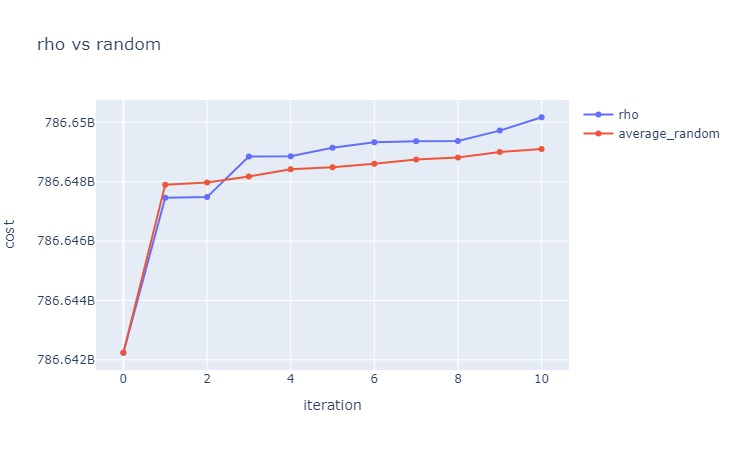
\includegraphics[width=1.1\textwidth]{images/rho_vas_average2.png}

In the subsequent plot, we compare the cost variation at each iteration using the validation function for interval refinement against the random interval selection method. The results indicate that the former method yields a significantly faster cost reduction, implying quicker convergence to the optimal solution. However, this approach incurs greater computational time, indicated as \textcolor{red}{many seconds s}. It is worth noting that while both the \(\rho\) and random iteration methods continue even upon encountering a feasible solution for the original problem, the validation function iteration may halt before reaching the maximum iteration limit if the current solution is feasible, thereby being optimal for the original problem.
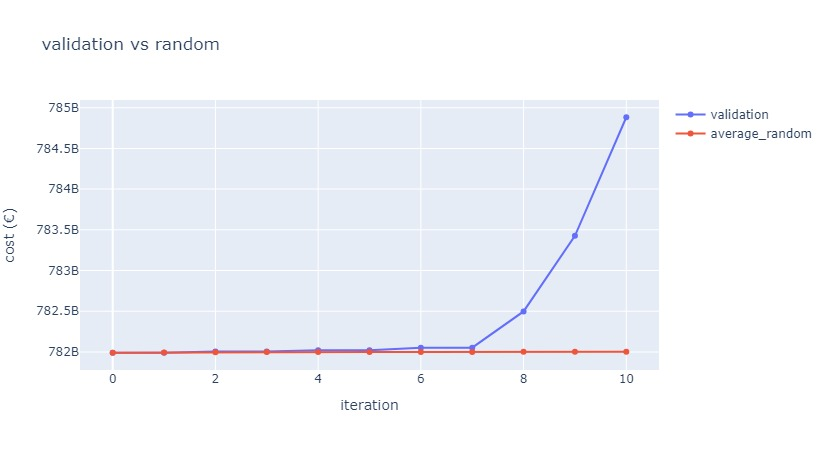
\includegraphics[width=\textwidth]{images/val_vs_average2.png}

\subsection{SINGLE NODE NETWORK}
First, an electrical grid with a single node is considered (corresponding ideally to an area with uniform
weather conditions, highly connected at low cost). A first section will consider realistic parameter
combinations and describe the results given by the solver, conducting a parameter sensitivity analysis. A
second section will describe a validation function that checks the results of the capacity expansion
problem for feasibility on new scenarios. Concurrently, a cost function is designed to give more realistic
cost estimates compared to the optimal value given by the solver.
\subsection{MULTIPLE NODE NETWORK}
Results are computed for a multiple node network, with additional edge variables and parameters. When
considering a network with more than a single node, computational costs increase rapidly. Thus in the
first section, a small analysis is carried out to determine acceptable time steps on which time dependent
data can be aggregated (the gathered data is usually on hourly steps) while maintaining the quality of the
solution. Some examples are then considered, and the network dynamics that arise with the introduction
of edge variables are described. A mixed approach is then used to design a validation function that can
deal with the complexity arising from the introduction of the network structure in the model.
\section{CONCLUSIONS}

%\begin{acknowledgements}
%If you'd like to thank anyone, place your comments here
%and remove the percent signs.
%\end{acknowledgements}


% Authors must disclose all relationships or interests that 
% could have direct or potential influence or impart bias on 
% the work: 
%
% \section*{Conflict of interest}
%
% The authors declare that they have no conflict of interest.


% BibTeX users please use one of
%bibliographystyle{spbasic}      % basic style, author-year citations
%\bibliographystyle{spmpsci}      % mathematics and physical sciences
%\bibliographystyle{spphys}       % APS-like style for physics
%\bibliography{sample}   % name your BibTeX data base

%\printbibliography[
%heading=bibintoc,
%title={Bibliography}]

% % Non-BibTeX users please use
\begin{thebibliography}{}
% %
% % and use \bibitem to create references. Consult the Instructions
% % for authors for reference list style.
% %
% \bibitem{RefJ}
% % Format for Journal Reference
% Author, Article title, Journal, Volume, page numbers (year)
% % Format for books
% \bibitem{RefB}
% Author, Book title, page numbers. Publisher, place (year)
% % etc

\bibitem{review_math_opt}
Michal Jasinski, Arsalan Najafi, et al,
Operation and Planning of Energy Hubs Under Uncertainty - A Review of Mathematical Optimization Approaches,
2022


\bibitem{European_H2_Market_landscape}
Author, European Hydrogen Market Landscape - November 2023 Report, page numbers. Publisher, place (year)


\bibitem{30y_gen}
Stefan Pfenninger and Iain Staffell. “Long-term patterns of European PV output us-
ing 30 years of validated hourly reanalysis and satellite data”. In: Energy 114 (2016),
pp. 1251–1265. issn: 0360-5442. doi: https://doi.org/10.1016/j.energy.2016.08.
060.

\bibitem{Gurobi}
Gurobi Optimization, LLC: Gurobi Optimizer Reference Manual (2024). https://www.gurobi.com

% %@article{European_H2_Market_landscape,
% %title = {European Hydrogen Market Landscape - November 2023 Report},
% % journal = {European Journal of Operational Research},
% % volume = {},
% % number = {1},
% % pages = {},
% % year = {2023},
% % doi = {},
% % url = {https://observatory.clean-hydrogen.europa.eu/sites/default/files/2023-11/Report%2001%20-%20November%202023%20-%20The%20European%20hydrogen%20market%20landscape.pdf},
% % author = {European Hydrogen Observatory},
% % keywords = {},
% % abstract = {}
% % }

% \bibitem{WindDataSet}
% Author, Book Title, page numbers. Publisher, place (year)

% % @article{WindDataSet,
% % title = {Using bias-corrected reanalysis to simulate current and future wind power output},
% % journal = {Energy},
% % volume = {114},
% % pages = {1224-1239},
% % year = {2016},
% % issn = {0360-5442},
% % doi = {https://doi.org/10.1016/j.energy.2016.08.068},
% % url = {https://www.sciencedirect.com/science/article/pii/S0360544216311811},
% % author = {Iain Staffell and Stefan Pfenninger},
% % keywords = {Wind power, Wind farm, Reanalysis, Capacity factor, Energy yield, Europe},
% % abstract = {Reanalysis models are rapidly gaining popularity for simulating wind power output due to their convenience and global coverage. However, they should only be relied upon once thoroughly proven. This paper reports the first international validation of reanalysis for wind energy, testing NASA's MERRA and MERRA-2 in 23 European countries. Both reanalyses suffer significant spatial bias, overestimating wind output by 50% in northwest Europe and underestimating by 30% in the Mediterranean. We derive national correction factors, and show that after calibration national hourly output can be modelled with R2 above 0.95. Our underlying data are made freely available to aid future research. We then assess Europe's wind resources with twenty-year simulations of the current and potential future fleets. Europe's current average capacity factor is 24.2%, with countries ranging from 19.5% (Germany) to 32.4% (Britain). Capacity factors are rising due to improving technology and locations; for example, Britain's wind fleet is now 23% more productive than in 2005. Based on the current planning pipeline, we estimate Europe's average capacity factor could increase by nearly a third to 31.3%. Countries with large stakes in the North Sea will see significant gains, with Britain's average capacity factor rising to 39.4% and Germany's to 29.1%.}
% % }


% \bibitem{PVDataSet}
% Author, Book Title, page numbers. Publisher, place (year)
% % @article{PVDataSet,
% % title = {Long-term patterns of European PV output using 30 years of validated hourly reanalysis and satellite data},
% % journal = {Energy},
% % volume = {114},
% % pages = {1251-1265},
% % year = {2016},
% % issn = {0360-5442},
% % doi = {https://doi.org/10.1016/j.energy.2016.08.060},
% % url = {https://www.sciencedirect.com/science/article/pii/S0360544216311744},
% % author = {Stefan Pfenninger and Iain Staffell},
% % keywords = {Solar energy, Meteorological reanalysis, Satellite irradiance estimation, Renewables, Grid integration of renewables},
% % abstract = {Solar PV is rapidly growing globally, creating difficult questions around how to efficiently integrate it into national electricity grids. Its time-varying power output is difficult to model credibly because it depends on complex and variable weather systems, leading to difficulty in understanding its potential and limitations. We demonstrate how the MERRA and MERRA-2 global meteorological reanalyses as well as the Meteosat-based CM-SAF SARAH satellite dataset can be used to produce hourly PV simulations across Europe. To validate these simulations, we gather metered time series from more than 1000 PV systems as well as national aggregate output reported by transmission network operators. We find slightly better accuracy from satellite data, but greater stability from reanalysis data. We correct for systematic bias by matching our simulations to the mean bias in modeling individual sites, then examine the long-term patterns, variability and correlation with power demand across Europe, using thirty years of simulated outputs. The results quantify how the increasing deployment of PV substantially changes net power demand and affects system adequacy and ramping requirements, with heterogeneous impacts across different European countries. The simulation code and the hourly simulations for all European countries are available freely via an interactive web platform, www.renewables.ninja.}
% % }


% \bibitem{Dunkelflaut}
% Author, Book Title, page numbers. Publisher, place (year)
% % @Article{Dunkelflaut,
% % AUTHOR = {Li, Bowen and Basu, Sukanta and Watson, Simon J. and Russchenberg, Herman W. J.},
% % TITLE = {A Brief Climatology of Dunkelflaute Events over and Surrounding the North and Baltic Sea Areas},
% % JOURNAL = {Energies},
% % VOLUME = {14},
% % YEAR = {2021},
% % NUMBER = {20},
% % ARTICLE-NUMBER = {6508},
% % URL = {https://www.mdpi.com/1996-1073/14/20/6508},
% % ISSN = {1996-1073},
% % DOI = {10.3390/en14206508}
% % }



% \bibitem{betaPV}
% Author, Book Title, page numbers. Publisher, place (year)
% % @article{betaPV,
% % title = {Prediction interval of wind power using parameter optimized Beta distribution based LSTM model},
% % journal = {Applied Soft Computing},
% % volume = {82},
% % pages = {105550},
% % year = {2019},
% % issn = {1568-4946},
% % doi = {https://doi.org/10.1016/j.asoc.2019.105550},
% % url = {https://www.sciencedirect.com/science/article/pii/S1568494619303308},
% % author = {Xiaohui Yuan and Chen Chen and Min Jiang and Yanbin Yuan},
% % keywords = {Wind power, Prediction interval, Long short-term memory neural network, Beta distribution, Particle swarm optimization},
% % abstract = {Prediction interval of wind power (PIWP) is crucial to assessing the economic and safe operation of the wind turbine and providing support for analysis of the stability of power systems. The hybrid model (Beta-PSO-LSTM) of long short-term memory (LSTM) neural network and Beta distribution function based particle swarm optimization (PSO) is put forward for prediction interval of wind power. In order to enhance the performance of the Beta-PSO-LSTM for PIWP in training process, wind power series are divided into different power intervals, and then the Beta-PSO-LSTM is used to estimate each power interval of the original wind power series. Furthermore, based on the analysis of the interval forecasting error information in wind power training data set, Beta distribution model is proposed to get better PIWP, and PSO is used to optimize the parameters of the model. Finally, the proposed Beta-PSO-LSTM model is compared with the Beta distribution optimized by PSO based the BP neural network (Beta-PSO-BP), the normal distribution based LSTM neural network (Norm-LSTM), Beta distribution based LSTM neural network (Beta-LSTM), and Beta distribution optimized by iterative method based LSTM neural network (Beta-IM-LSTM) for PIWP. The simulation results show that the PIWP obtained by the Beta-PSO-LSTM model has higher reliability and narrower interval bandwidth, which can provide decision support for the safe and stable operation of power systems.}
% % }


% \bibitem{GaussCopula}
% Author, Book Title, page numbers. Publisher, place (year)
% % @ARTICLE{GaussCoupula,
% %   author={Papaefthymiou, George and Kurowicka, Dorota},
% %   journal={IEEE Transactions on Power Systems}, 
% %   title={Using Copulas for Modeling Stochastic Dependence in Power System Uncertainty Analysis}, 
% %   year={2009},
% %   volume={24},
% %   number={1},
% %   pages={40-49},
% %   keywords={Power system modeling;Stochastic systems;Power system analysis computing;Uncertainty;Random variables;Power system planning;Stochastic processes;Power generation;Context modeling;Aggregates;Copula;correlation;Monte Carlo simulation;stochastic dependence;stochastic generation;uncertainty analysis;wind power},
% %   doi={10.1109/TPWRS.2008.2004728}}


% \bibitem{weibullwind}
% Author, Book Title, page numbers. Publisher, place (year)
% % @article{weibullwind,
% % title = {Evaluation of wind power production prospective and Weibull parameter estimation methods for Babaurband, Sindh Pakistan},
% % journal = {Energy Conversion and Management},
% % volume = {78},
% % pages = {956-967},
% % year = {2014},
% % issn = {0196-8904},
% % doi = {https://doi.org/10.1016/j.enconman.2013.06.062},
% % url = {https://www.sciencedirect.com/science/article/pii/S019689041300589X},
% % author = {Shahnawaz Farhan Khahro and Kavita Tabbassum and Amir Mahmood Soomro and Lei Dong and Xiaozhong Liao},
% % keywords = {Wind energy, Power density function, Weibull distribution, Frequency distribution, Wind rose},
% % abstract = {Pakistan is currently experiencing an acute shortage of energy and urgently needs new sources of affordable energy that could alleviate the misery of the energy starved masses. At present the government is increasing not only the conventional energy sources like hydel and thermal but also focusing on the immense potential of renewable energy sources like; solar, wind, biogas, waste-to-energy etc. The recent economic crisis worldwide, global warming and climate change have also emphasized the need for utilizing economic feasible energy sources having lowest carbon emissions. Wind energy, with its sustainability and low environmental impact, is highly prominent. The aim of this paper is to explore the wind power production prospective of one of the sites in south region of Pakistan. It is worth mentioning here that this type of detailed analysis is hardly done for any location in Pakistan. Wind power densities and frequency distributions of wind speed at four different altitudes along with estimated wind power expected to be generated through commercial wind turbines is calculated. Analysis and comparison of 5 numerical methods is presented in this paper to determine the Weibull scale and shape parameters for the available wind data. The yearly mean wind speed of the considered site is 6.712m/s and has power density of 310W/m2 at 80m height with high power density during April to August (highest in May with wind speed 9.595m/s and power density 732W/m2). Economic evaluation, to exemplify feasibility of installing wind turbines, is also done. The estimated cost of per kWh of electricity from wind is calculated as 0.0263US$/kWh. Thus the candidate site is recommended for some small stand-alone systems as well as for wind farm.}
% % }


% \bibitem{future_climate}
% Author, Book Title, page numbers. Publisher, place (year)
% % @article{future_climate,
% %     author = {Bett, P. E., Thornton, H. E., and Clark, R. T.},
% %     title = {European wind variability over 140 yr},
% %     journal = {Adv. Sci. Res., 10, 51–58},
% %     year = {2013}
% % }




\end{thebibliography}

\end{document}
% end of file template.tex

